\documentclass[10pt]{article}
\usepackage[polish]{babel}
\usepackage[utf8]{inputenc}
\usepackage[T1]{fontenc}
\usepackage{amsmath}
\usepackage{amsfonts}
\usepackage{amssymb}
\usepackage[version=4]{mhchem}
\usepackage{stmaryrd}
\usepackage{bbold}
\usepackage{graphicx}
\usepackage[export]{adjustbox}
\graphicspath{ {./images/} }

\title{PRACA KONTROLNA nr 1 - POZIOM PODSTAWOWY }

\author{}
\date{}


\begin{document}
\maketitle
\begin{enumerate}
  \item Ile jest trzycyfrowych liczb naturalnych:\\
a) podzielnych przez 3 lub przez 5?\\
b) podzielnych przez 3 lub przez 6?\\
c) podzielnych przez 3 i niepodzielnych przez 5?
  \item Renomowany dom mody sprzedał $40 \%$ kolekcji letniej po założonej cenie. Po obniżce ceny o $50 \%$ udało się sprzedać połowę pozostałej części towaru i dopiero kolejna $50 \%$ owa obniżka pozwoliła opróżnić magazyny. Ile procent zaplanowanego przychodu stanowi uzyskana ze sprzedaży kwota? O ile procent wyjściowa cena towaru powinna była być wyższa, by sklep uzyskał zaplanowany początkowo przychód?
  \item Określić dziedzinę wyrażenia $w(x, y)=\frac{2}{x-y}-\frac{3 x y}{x^{3}-y^{3}}-\frac{x-y}{x^{2}+x y+y^{2}}$. Sprowadzić je do najprostszej postaci i obliczyć $w\left(1+\sqrt{2},(1+\sqrt{2})^{-1}\right)$.
  \item Obliczyć sumę wszystkich liczb pierwszych spełniających nierówność
\end{enumerate}

$$
(p-4) x^{2}-4(p-2) x-p \leqslant 0, \quad \text { gdzie } \quad p=\frac{64^{\frac{1}{3}} \sqrt{8}+8^{\frac{1}{3}} \sqrt{64}}{\sqrt[3]{64 \sqrt{8}}}
$$

\begin{enumerate}
  \setcounter{enumi}{4}
  \item Dwa naczynia zawierają w sumie 40 litrów wody. Po przelaniu pewnej części wody pierwszego naczynia do drugiego, w pierwszym naczyniu zostało trzy razy mniej wody niż w drugim. Gdy następnie przelano taką samą część wody drugiego naczynia do pierwszego, okazało się, że w obu naczyniach jest tyle samo płynu. Obliczyć, ile wody było pierwotnie w każdym naczyniu i jaką jej część przelewano.
  \item Dwie gaździny, pracując razem, mogą wykonać zamówioną partię pisanek w ciągu 7 dni pod warunkiem, że pierwsza z nich rozpocznie pracę o półtora dnia wcześniej niż druga. Gdyby każda z nich pracowała oddzielnie, to druga wykonałaby całą pracę o 3 dni wcześniej od pierwszej. Ile dni potrzebuje każda z kobiet na wykonanie całej pracy?
\end{enumerate}

\section*{PRACA KONTROLNA nr 1 - POZIOM ROZSZERZONY}
\begin{enumerate}
  \item Ile jest liczb pięciocyfrowych podzielnych przez 9 , które w rozwinięciu dziesiętnym mają: a) obie cyfry 1,2 i tylko te? b) obie cyfry 1,3 i tylko te? c) wszystkie cyfry $1,2,3$ i tylko te? Odpowiedź uzasadnić. W przypadku b) wypisać otrzymane liczby.
  \item Pan Kowalski zaciągnął 31 grudnia pożyczkę 4000 złotych oprocentowaną w wysokości $18 \%$ w skali roku. Zobowiązał się spłacić ją w ciągu roku w trzech równych ratach płatnych 30 kwietnia, 30 sierpnia i 30 grudnia. Oprocentowanie pożyczki liczy się od 1 stycznia, a odsetki od kredytu naliczane są w terminach płatności rat. Obliczyć wysokość tych rat w zaokragleniu do pełnych groszy.
  \item Określić dziedzinę wyrażenia\\
$w(x, y)=\frac{x}{x^{3}+x^{2} y+x y^{2}+y^{3}}+\frac{y}{x^{3}-x^{2} y+x y^{2}-y^{3}}+\frac{1}{x^{2}-y^{2}}-\frac{1}{x^{2}+y^{2}}-\frac{x^{2}+2 y^{2}}{x^{4}-y^{4}}$.\\
Sprowadzić je do najprostszej postaci i obliczyć $w\left(\cos 15^{\circ}, \sin 15^{\circ}\right)$.
  \item Liczba $p=\frac{(\sqrt[3]{54}-2)(9 \sqrt[3]{4}+6 \sqrt[3]{2}+4)-(2-\sqrt{3})^{3}}{\sqrt{3}+(1+\sqrt{3})^{2}}$ jest miejscem zerowym funkcji kwadratowej $f(x)=a x^{2}+b x+c$. Wyznaczyć współczynniki $a, b, c$ oraz drugie miejsce zerowe tej funkcji wiedząc, że największą wartością funkcji jest 4, a jej wykres jest symetryczny względem prostej $x=1$.
  \item Do zbiornika poprowadzono trzy rury. Pierwsza rura potrzebuje do napełnienia zbiornika o 4 godziny więcej niż druga, a trzecia napełnia cały zbiornik w czasie dwa razy krótszym niż pierwsza. W jakim czasie napełnia zbiornik każda z rur, jeżeli wiadomo, że wszystkie trzy rury otwarte jednocześnie napełniają zbiornik w ciągu 2 godzin i 40 minut?
  \item Z przystani A wyrusza z biegiem rzeki statek do przystani B, odległej od A o 140 km . Po upływie 1 godziny wyrusza za nim łódź motorowa, dopędza statek, po czym wraca do przystani A w tym samym momencie, w którym statek przybija do przystani B. Znaleźć prędkość biegu rzeki, jeżeli wiadomo, że w stojącej wodzie prędkość statku wynosi 16 km/godz, a prędkość łodzi 24 km/godz.
\end{enumerate}

\section*{PRACA KONTROLNA nr 2 - POZIOM PODSTAWOWY}
\begin{enumerate}
  \item Niech $A=\left\{x \in \mathbb{R}: \frac{1}{x^{2}+23} \geqslant \frac{1}{10 x}\right\}$ oraz $B=\left\{x \in \mathbb{R}:|x-2|<\frac{7}{2}\right\}$.
\end{enumerate}

Zbiory $A, B, A \cup B, A \cap B, A \backslash B$ i $B \backslash A$ zapisać w postaci przedziałón liczbowych i zaznaczyć je na osi liczbowej.\\
2. Zaznaczyć na płaszczyźnie zbiory

$$
A=\{(x, y):|x|+|y| \leqslant 2\} \quad \text { oraz } \quad B=\left\{(x, y): \frac{1}{|x-1|} \leqslant \frac{1}{|x+3|}, \frac{2}{|y-1|} \geqslant 1\right\}
$$

i obliczyć pole zbioru $A \cap B$.\\
3. Trójmian kwadratowy $f(x)=a x^{2}+b x+c$ przyjmuje najmniejszą wartość równą -1 w punkcie $x=1$ a reszta z dzielenia tego trójmianu przez dwumian ( $x-2$ ) równa jest 1. Wyznaczyć współczynniki $a, b, c$. Narysować staranny wykres funkcji $g(x)=f(|x|)$ i wyznaczyć najmniejszą i największą wartość tej funkcji na przedziale[-1,3].\\
4. Tangens kąta ostrego $\alpha$ równy jest $\frac{a}{b}$, gdzie

$$
a=(\sqrt{2+\sqrt{3}}-\sqrt{2-\sqrt{3}})^{2}, \quad b=(\sqrt{\sqrt{2}+1}-\sqrt{\sqrt{2}-1})^{2} .
$$

Wyznaczyć wartości pozostałych funkcji trygonometrycznych tego kąta. Wykorzystując wzór $\sin 2 \alpha=2 \sin \alpha \cos \alpha$, obliczyć miarę kąta $\alpha$.\\
5. Narysować wykres funkcji $f(x)=\sqrt{4 x^{2}-4 x+1}-x$ i rozwiązać nierówność $f(x)<0$. W zależności od parametru $m$ określić liczbę rozwiązań równania $|f(x)|=m$. Dla jakiego $a$ pole trójkąta ograniczonego osią $O x$ i wykresem funkcji $g(x)=f(x)-a$ równe jest 6?\\
6. Niech $f(x)=\left\{\begin{array}{rll}x^{2}+2 x & \text { dla } & x \leqslant 1, \\ 2+\frac{1}{x} & \text { dla } & x>1 .\end{array}\right.$\\
a) Narysować wykres funkcji $f$ i na jego podstawie wyznaczyć zbiór wartości funkcji.\\
b) Obliczyć $f(\sqrt{3}-1)$ oraz $f(3-\sqrt{3})$.\\
c) Rozwiązać nierówność $2 \sqrt{f(x)} \leqslant 3$ i zbiór jej rozwiązań zaznaczyć na osi $0 x$.

\section*{PRACA KONTROLNA nr 2 - POZIOM ROZSZERZONY}
\begin{enumerate}
  \item Rozwiązać nierówność $\frac{1}{\sqrt{5+4 x-x^{2}}} \geqslant \frac{1}{x-2}$ i zbiór rozwiązań zaznaczyć na prostej.
  \item Niech $A=\{(x, y): y \geqslant||x-2|-1|\}, B=\left\{(x, y): y+\sqrt{4 x-x^{2}-3} \leqslant 2\right\}$.
\end{enumerate}

Narysować na płaszczyźnie zbiór $A \cap B$ i obliczyć jego pole.\\
3. Dla jakich wartości rzeczywistego parametru $p$ równanie $(p-1) x^{4}+(p-2) x^{2}+p=0$ ma dokładnie dwa różne pierwiastki?\\
4. Znaleźć wszystkie wartości parametru rzeczywistego $m$, dla których pierwiastki trójmianu kwadratowego $f(x)=(m-2) x^{2}-(m+1) x-m$ spełniają nierówność $\left|x_{1}\right|+\left|x_{2}\right| \leqslant 1$.\\
5. Narysować staranny wykres funkcji

$$
f(x)=\left\{\begin{array}{rll}
\sqrt{x^{2}-4 x+4}-1 & , \text { gdy } & |x-2| \geqslant 1 \\
-\sqrt{4 x-x^{2}-3} & , \text { gdy } & |x-2| \leqslant 1
\end{array}\right.
$$

i rozwiązać nierówność $|f(x)|>\frac{1}{2}$. W zależności od parametru $m$ określić liczbę rozwiązań równania $|f(x)|=m$. Obliczyć pole obszaru ograniczonego wykresem funkcji $g(x)=|f(x)|$ i prostą $y=\frac{1}{2}$.\\
6. Niech

$$
f(x)=\left\{\begin{array}{lll}
\frac{1}{x-1}, & \text { gdy } & |x-1| \geqslant 1 \\
x^{2}-x-1, & \text { gdy } & |x-1|<1
\end{array}\right.
$$

a) Obliczyć $f\left(-\frac{2}{3}\right), f\left(\frac{1+\sqrt{3}}{2}\right)$ oraz $f(\pi-1)$.\\
b) Narysować wykres funkcji $f$ i na jego podstawie podać zbiór wartości funkcji.\\
c) Rozwiązać nierówność $f(x) \geqslant-\frac{1}{2}$ i zaznaczyć na osi $0 x$ zbiór jej rozwiązań.

\section*{PRACA KONTROLNA nr 3 - POZIOM PODSTAWOWY}
\begin{enumerate}
  \item W trójkącie prostokątnym o kącie prostym przy wierzchoku $C$ na przedłużeniu przeciwprostokątnej $A B$ odmierzono odcinek $B D$ tak, że $|B D|=|B C|$. Wyznaczyć $|C D|$ oraz obliczyć pole trójkta $\triangle A C D$, jeżeli $|B C|=5,|A C|=12$.
  \item Harcerze rozbili 2 namioty, jeden w odległości 5 m , drugi - 17 m od prostoliniowego brzegu rzeki. Odległość między namiotami równa jest 13 m . W którym miejscu na samym brzegu rzeki (licząc od punktu brzegu będącego rzutem prostopadłym punktu położenia pierwszego namiotu) powinni umieścić maszt z flagą zastępu, by odległość od masztu do każdego z namiotów była taka sama?
  \item Na kole o promieniu $r$ opisano trapez równoramienny, w którym stosunek długości podstaw wynosi $4: 3$. Obliczyć stosunek pola koła do pola trapezu oraz cosinus kąta ostrego w tym trapezie.
  \item Wielomian $W(x)=x^{3}-x^{2}+b x+c$ jest podzielny przez $(x+3)$, a reszta z dzielenia tego wielomianu przez $(x-3)$ równa jest 6 . Wyznaczyć $b$ i $c$, a następnie rozwiązać nierówność $(x+1) W(x-1)-(x+2) W(x-2) \leqslant 0$.
  \item Wykonać działania i zapisać w najprostszej postaci wyrażenie
\end{enumerate}

$$
s(a, b)=\left(\frac{a^{2}+b^{2}}{a^{2}-b^{2}}-\frac{a^{3}+b^{3}}{a^{3}-b^{3}}\right):\left(\frac{a^{2}}{a^{3}-b^{3}}-\frac{a}{a^{2}+a b+b^{2}}\right) .
$$

Wyznaczyć wysokość trójkąta prostokątnego wpisanego w okrąg o promieniu 6 opuszczoną z wierzchołka kąta prostego wiedząc, że tangens jednego z kątów ostrych tego trójkąta równy jest $s(\sqrt{5}+\sqrt{3}, \sqrt{5}-\sqrt{3})$.\\
6. W trójkącie $A B C$ dane są $\angle C A B=\frac{\pi}{3}$, wysokość $|C D|=h=5$ oraz $B D=d=\sqrt{2}$. Obliczyć odległość środków okręgów wpisanych w trójkąty ADC i DBC.

\section*{PRACA KONTROLNA nr 3 - POZIOM ROZSZERZONY}
\begin{enumerate}
  \item Dany jest wielomian $W(x)=x^{3}+a x+b$, gdzie $b \neq 0$. Wykazać, że $W(x)$ posiada pierwiastek podwójny wtedy i tylko wtedy, gdy spełniony jest warunek $4 a^{3}+27 b^{2}=0$. Wyrazić pierwiastki za pomocą współczynnika $b$.
  \item Wyznaczyć promień okręgu opisanego na czworokącie $A B C D$, w którym kąt przy wierzchołku $A$ ma miarę $\alpha$, kąty przy wierzchołkach $B, D$ są proste oraz $|B C|=a,|A D|=b$. Sporządzić staranny rysunek.
  \item Narysować staranny wykres funkcji $f(x)=\frac{\sin 2 x-|\sin x|}{\sin x}$. W przedziale $[0, \pi]$ wyznaczyć rozwiązania nierówności $f(x)<2(\sqrt{2}-1) \cos ^{2} x$.
  \item Z wierzchołka $A$ kwadratu $A B C D$ o boku $a$ poprowadzono dwie proste, które dzielą kąt przy tym wierzchołku na trzy równe części i przecinają boki kwadratu w punktach $K$ i L. Wyznaczyć długości odcinków, na jakie te proste dzielą przekątną kwadratu. Znaleźć promień okręgu wpisanego w deltoid $A K C L$.
  \item Czworokąt wypukły $A B C D$, w którym $A B=1, B C=2, C D=4, D A=3$ jest wpisany w okrąg. Obliczyć promień $R$ tego okręgu. Sprawdzić, czy w czworokąt ten można wpisać okrąg. Jeżeli tak, to obliczyć promień $r$ tego okręgu.
  \item Na boku $B C$ trójkąta równobocznego obrano punkt $D$ tak, że promień okręgu wpisanego w trójkąt $A D C$ jest dwa razy mniejszy niż promień okręgu wpisanego w trójkąt $A B D$. W jakim stosunku punkt $D$ dzieli bok $B C$ ?
\end{enumerate}

\section*{PRACA KONTROLNA nr 4 - POZIOM PODSTAWOWy}
\begin{enumerate}
  \item Rozwiązać równanie $\frac{1}{\cos x}+\operatorname{tg} x-\sin \left(\frac{\pi}{2}-x\right)=0$ dla $x \in[-2 \pi, 2 \pi]$.
  \item Na płaszczyźnie dane są cztery punkty: $A(1,-1), B(5,7), C(4,-4), D(2,4)$. Obliczyć odległość punktu przecięcia prostych $A B$ i $C D$ od symetralnej odcinka $B C$. Sporządzić rysunek.
  \item Rozwiązać układ równań
\end{enumerate}

$$
\left\{\begin{array}{l}
y+x^{2}=4 \\
4 x^{2}-y^{2}+2 y=1
\end{array}\right.
$$

Podać interpretację geometryczną tego układu i wykazać, że cztery punkty, które są jego rozwiązaniem, wyznaczają na płaszczyźnie trapez równoramienny. Znaleźć równanie okręgu opisanego na tym trapezie.\\
4. W ostrosłupie prawidłowym trójkątnym długość krawędzi podstawy jest równa $a$. Kąt między krawędzią podstawy, a krawędzią boczną jest równy $\frac{\pi}{4}$. Obliczyć pole przekroju ostrosłupa płaszczyzną przechodzącą przez krawędź podstawy i środek przeciwległej krawędzi bocznej. Sporządzić staranny rysunek.\\
5. Dane są dwa okręgi: $K_{1}$ o środku w punkcie $(0,0)$ i promieniu 5 i $K_{2}$ o równaniu $x^{2}+6 x+y^{2}-12 y+5=0$. Obliczyć pole czworokąta wyznaczonego przez środki okręgów oraz punkty, w których te okręgi się przecinają. Sporządzić staranny rysunek.\\
6. Podstawą graniastosłupa jest równoległobok o bokach długości $a$ i $2 a$ oraz kącie ostrym $\frac{\pi}{3}$. Krótsza przekątna graniastosłupa tworzy w płaszczyzną podstawy kąt $\frac{\pi}{6}$. Obliczyć długość dłuższej przekątnej oraz pole powierzchni całkowitej tego graniastosłupa.

\section*{PRACA KONTROLNA nr 4 - POZIOM ROZSZERZONY}
\begin{enumerate}
  \item Rozwiązać równanie $2 \sin ^{2} x-2 \sin x \cos 2 x=1$.
  \item Dane są dwa wektory $\vec{a}=[2,-3]$ oraz $\vec{b}=[-1,4]$. Pokazać, że wektor $\overrightarrow{A B}=3 \vec{a}+2 \vec{b}$ jest prostopadły do wektora $\overrightarrow{B C}=8 \vec{a}+11 \vec{b}$. Obliczyć długość środkowej trójkąta $A B C$ rozpiętego na wektorach $\overrightarrow{A B}$ i $\overrightarrow{B C}$, poprowadzonej z wierzchołka $B$.
  \item Niech $K$ będzie wierzchołkiem paraboli $f(x)=-\frac{4}{9} x^{2}-\frac{8}{3} x$, a $L$ - wierzchołkiem paraboli $g(x)=-f(x-7)+7$. Na paraboli $g(x)$ znaleźć taki punkt $N$, aby wektor $\overrightarrow{N L}$ był równoległy do wektora $\overrightarrow{M K}$, gdzie $M=(0, f(0))$. Obliczyć pole czworokąta $K M L N$.
  \item Przekrój sześcianu płaszczyzną jest sześciokątem foremnym. Wyznaczyć kąt nachylenia tej płaszczyzny do płaszczyzny podstawy sześcianu oraz obliczyć pole tego przekroju. Wykonać odpowiedni rysunek.
  \item Dane są dwa okręgi: $K_{1}$ o środku w punkcie $P(1,1)$ i promieniu 1 oraz $K_{2}$ o środku $Q(9,5)$ i promieniu 3. Znaleźć punkt $S$ na odcinku $\overline{P Q}$ oraz dobrać skalę $k$ tak, aby okrąg $K_{2}$ był obrazem okręgu $K_{1}$ w jednokładności o środku $S$ i skali $k$. Wyznaczyć równania prostych, które są styczne jednocześnie do obu okręgów i przechodzą przez punkt $S$.
  \item W ostrosłupie prawidłowym czworokątnym pole każdej z pięciu ścian jest równe 1. Ostrosłup ten ścięto w połowie wysokości płaszczyzną równoległą do podstawy. Obliczyć objętość oraz pole powierzchni całkowitej otrzymanego ostrosłupa ściętego. Wykonać odpowiedni rysunek.
\end{enumerate}

\section*{PRACA KONTROLNA nr 5 - POZIOM PODSTAWOWY}
\begin{enumerate}
  \item W ciągu arytmetycznym suma początkowych dwudziestu jeden wyrazów wynosi $21 \sqrt{2}$, a jego dziesiąty wyraz równy jest $-2-2 \sqrt{2}$. Wyznaczyć najmniejszy dodatni wyraz tego ciągu.
  \item Rozwiązać nierówność
\end{enumerate}

$$
-2<\log _{\frac{1}{2}}(5 x+2) \leqslant 2
$$

\begin{enumerate}
  \setcounter{enumi}{2}
  \item Firmy X i Y jednocześnie rozpoczęły działalność. W pierwszym miesiącu każda z nich miała dochód równy $50000 \mathrm{zł}$. Po pięciu miesiącach okazało sie, że dochód firmy X rósł z miesiąca na miesiąc o tę samą kwotę, a dochód firmy Y wzrastał co miesiąc geometrycznie. W drugim i trzecim miesiącu działalnosci firma X miała dochód wiekszy od dochodu firmy Y o 2000 zł. Ustalić, która z firm miała wiekszą sumę dochodów w pierwszych pięciu miesiącach swojej działalności.
  \item Sporządzić staranny wykres funkcji (za jednostkę przyjąć 2 cm )
\end{enumerate}

$$
f(x)=\left\{\begin{array}{lll}
\frac{|x|}{1-x} & \text { dla } & |x-1| \geqslant 1 \\
-2 x^{2}+3 x & \text { dla } & |x-1|<1
\end{array}\right.
$$

Korzystając z niego, określić ilość rozwiązań równania $f(x)=m$ w zależności od rzeczywistego parametru $m$.\\
5. Stosując wzór na sinus podwojonego kąta oraz wzory redukcyjne, obliczyć wartość wyrażenia

$$
\cos \frac{\pi}{5} \cdot \cos \frac{2 \pi}{5} \cdot \cos \frac{3 \pi}{5} \cdot \cos \frac{4 \pi}{5}
$$

\begin{enumerate}
  \setcounter{enumi}{5}
  \item Wiedząc, że $\sin \frac{\pi}{10}=\frac{1}{4}(\sqrt{5}-1)$, wyznaczyć wszystkie kąty $\alpha \in[0, \pi]$, dla których spełnione jest równanie
\end{enumerate}

$$
2^{2+\sin \alpha}=\sqrt{2} \cdot 4^{\cos ^{2} \alpha}
$$

\section*{PRACA KONTROLNA nr 5 - POZIOM ROZSZERZONY}
\begin{enumerate}
  \item Zaznaczyć na osi liczbowej zbiór rozwiązań nierówności
\end{enumerate}

$$
\frac{2 x-\sqrt{2-x}}{x} \geqslant x
$$

\begin{enumerate}
  \setcounter{enumi}{1}
  \item Wyznaczyć wszystkie liczby rzeczywiste $x$, dla których funkcja
\end{enumerate}

$$
f(x)=2^{x^{2}+2}-2^{x^{2}-1}-2 \cdot 7^{x^{2}-1}
$$

przyjmuje wartości dodatnie.\\
3. Określić dziedzinę i sporządzić staranny wykres funkcji $f(x)=1-\log _{3}(1-x)$. Za jednostkę przyjąć 2 cm . Znaleźć obraz tego wykresu w symetrii osiowej względem prostej $x=y$ i podać wzór funkcji, której wykresem jest nowo powstała krzywa.\\
4. Rozwiązać nierówność

$$
\sqrt{\log _{2}\left(x^{2}-1\right)}>\log _{2} \sqrt{x^{2}-1}
$$

\begin{enumerate}
  \setcounter{enumi}{4}
  \item Niech $c>0$ i $c \neq 1$. Znaleźć liczbę naturalną $m$, dla ktorej suma $m$ początkowych wyrazów ciągu arytmetycznego $a_{n}=\log _{2}\left(c^{n}\right)$, jest 10100 razy większa od sumy wszystkich wyrazów ciągu geometrycznego $b_{n}=\log _{2^{3^{n}}}(c)$.
  \item Korzystając ze wzoru
\end{enumerate}

$$
\sin 5 \alpha=5 \sin \alpha-20 \sin ^{3} \alpha+16 \sin ^{5} \alpha
$$

obliczyć wartość $\sin \frac{\pi}{5}$. Podać wartości wyrażeń $\cos \frac{\pi}{5}, \sin \frac{\pi}{10}$ oraz $\cos \frac{\pi}{10}$. Wyprowadzić wzór na pole dwudziestokąta foremnego wpisanego w okrąg o promieniu $r$.

\section*{PRACA KONTROLNA nr 6 - POZIOM PODSTAWOWY}
\begin{enumerate}
  \item Losujemy liczbę ze zbioru $\{1,2,3, \ldots, 100\}$, a następnie liczbę ze zbioru $\{2,3,4,5\}$. Obliczyć prawdopodobieństwo, że pierwsza z wylosowanych liczb jest podzielna przez drugą.
  \item Liczba 2-elementowych podzbiorów zbioru $A$ jest 7 razy większa niż liczba 2-elementowych podzbiorów zbioru $B$. Liczba 2-elementowych podzbiorów zbioru $A$ nie zawierających ustalonego elementu $a \in A$ jest 5 razy większa niż liczba 2-elementowych podzbiorów zbioru $B$. Ile elementów ma każdy z tych zbiorów? Ile każdy z tych zbiorów ma podzbiorów 3 -elementowych?
  \item W turnieju szachowym każdy uczestnik miał rozegrać z pozostałymi po jednej partii. Po rozegraniu trzech partii dwóch szachistów zrezygnowało z dalszej gry. W sumie rozegrano 84 partie. Ilu było uczestników na początku turnieju, jeżeli dwaj zawodnicy, którzy zrezygnowali, nie grali ze sobą?
  \item Suma pierwszego i trzeciego wyrazu ciągu geometrycznego $\left(a_{n}\right)$ wynosi 20. Znajdź wzór ogólny ciągu arytmetycznego ( $b_{n}$ ) takiego, że $b_{1}=a_{1}, b_{2}=a_{2}, b_{5}=a_{3}$.
  \item Rozkład ocen ze sprawdzianu w klasie IIIa jest opisany tabelką
\end{enumerate}

$$
\begin{array}{c|c|c|c|c|c}
\text { ocena } & 1 & 2 & 3 & 4 & 5 \\
\hline \text { liczba osób } & 1 & 2 & 8 & 9 & 6
\end{array}
$$

Jaś otrzymał ocenę 4. Czy wypadł powyżej średniej w swojej klasie? W pozostałych klasach średnie punktów wynosiły: 3,875 w IIIb (24 osoby) i 4,6 w IIIc (25 osób). Czy ocena otrzymana przez Jasia znajduje się powyżej średniej liczonej łącznie wśród wszystkich uczniów klas trzecich? Ile co najmniej, a ile co najwyżej, osób miało piątki w klasie IIIc (skala ocen to $1,2, \ldots, 5$ )?\\
6. Ile liczb czterocyfrowych o wszystkich cyfrach różnych można utworzyć z cyfr 1,2,3,4,5, a ile z cyfr 0,1,2,3,4,5,6? W obu przypadkach obliczyć, ile można utworzyć czterocyfrowych liczb podzielnych przez 5.

\section*{PRACA KONTROLNA nr 6 - POZIOM ROZSZERZONY}
\begin{enumerate}
  \item Trzeci składnik rozwinięcia dwumianu $\left(\sqrt[3]{x}+\frac{1}{\sqrt{x}}\right)^{n}$ ma współczynnik równy 45. Wyznaczyć wszystkie składniki tego rozwinięcia, w których $x$ występuje w potędze o wykładniku całkowitym.
  \item W turnieju szachowym rozgrywanym systemem „każdy z każdym" dwóch uczestników nie ukończyło turnieju, przy czym jeden z nich rozegrał 10 partii, a drugi tylko jedną. Ilu było zawodników i czy wspomniani zawodnicy grali ze sobą, jeżeli rozegrano 55 partii?
  \item W pudełku jest 400 kul w tym $n$ czerwonych. Wybieramy losowo dwie kule. Prawdopodobieństwo wylosowania dwóch kul czerwonych jest równe $\frac{1}{760}$.\\
a) Ile kul czerwonych jest w tym pudełku?\\
b) Obliczyć prawdopodobieństwo, że żadna z wylosowanych kul nie jest czerwona.
  \item Suma wyrazów nieskończonego ciągu geometrycznego zmniejszy się o $25 \%$, jeżeli wykreślimy z niej składniki o numerach parzystych niepodzielnych przez 4. Obliczyć sumę wszystkich wyrazów tego ciągu wiedząc, że jego drugi wyraz wynosi 1.
  \item Stosując zasadę indukcji matematycznej udowodnić prawdziwość wzoru
\end{enumerate}

$$
\binom{2}{2}-\binom{3}{2}+\binom{4}{2}-\binom{5}{2}+\ldots+\binom{2 n}{2}=n^{2}, n \geqslant 1 .
$$

\begin{enumerate}
  \setcounter{enumi}{5}
  \item Wśród wszystkich bliźniąt $64 \%$ stanowią bliźnięta tej samej płci. Prawdopodobieństwo urodzenia chłopca wynosi 0,51 . Obliczyć prawdopodobieństwo, że drugie z bliźniąt jest dziewczynką, pod warunkiem, że:\\
a) pierwsze jest dziewczynką,\\
b) pierwsze jest chłopcem.
\end{enumerate}

\section*{PRACA KONTROLNA nr 7 - POZIOM PODSTAWOWY}
\begin{enumerate}
  \item Rozwiązać równanie $1-|x|=\sqrt{1+x}$ i podać jego ilustrację graficzną.
  \item Wyznaczyć wszystkie punkty $x$ z przedziału $[0,2 \pi]$, dla których spełniona jest nierówność $\sin 2 x-\operatorname{tg} x \leqslant 0$. Podać ilustrację graficzną nierówności.
  \item Określić liczbę rozwiązań układu równań
\end{enumerate}

$$
\left\{\begin{array}{l}
y=|x-2|+1, \\
y=a x
\end{array}\right.
$$

w zależności od wartości współczynnika kierunkowego prostej $y=a x$. Znaleźć rozwiązania w przypadku, gdy jednym z nich jest para (4,3). Sporządzić staranny rysunek.\\
4. Dana jest prosta $l: x+2 y-4=0$. Przez punkt $(1,1)$ poprowadzić prostą $k$ o dodatnim współczynniku kierunkowym tak, aby pole trójkąta ograniczonego prostymi $l, k$ i osią $0 x$ było dwa razy większe niż pole trójkąta ograniczonego tymi prostymi i osią $0 y$.\\
5. Trójkąt równoboczny $A B C$ o boku długości a zgięto wzdłuż wysokości $C D$ pod pewnym kątem, otrzymując w ten sposób czworościan $A B C D$. Obliczyć objętość i pole powierzchni całkowitej tego czworościanu wiedząc, że tangens kąta nachylenia ściany $A B C$ do podstawy czworościanu równy jest $\sqrt{6}$.\\
6. Punkt $(0,2)$ jest środkiem symetrii wykresu funkcji $f(x)=x(|x|-2 a)+b$. Wyznaczyć $a$ i $b$ wiedząc, że $f(a)=0$.

\section*{PRACA KONTROLNA nr 7 - POZIOM ROZSZERZONY}
\begin{enumerate}
  \item Rozwiązać równanie
\end{enumerate}

$$
\sqrt{8+2 x-x^{2}}=2 x-5
$$

Zilustrować je odpowiednim wykresem.\\
2. Wyznaczyć wszystkie wartości parametru rzeczywistego $p$, dla których rozwiązania układu równań

$$
\left\{\begin{aligned}
p x+2 y & =\frac{p}{2} \\
2 x+p y & =p-1
\end{aligned}\right.
$$

są zawarte w kwadracie $K=\{(x, y):|x|+|y| \leqslant 1\}$.\\
3. Bok $A B$ trójkąta równoramiennego $A B C$ leży na prostej $l: x-3 y-4=0$. Punkt $D(4,0)$ jest spodkiem wysokości tego trójkąta, a $S(2,1)$ środkiem boku $A C$. Wyznaczyć współrzędne wierzchołka $B$. Sporządzić rysunek.\\
4. Podstawą ostrosłupa o wysokości $h$ jest trójkąt prostokątny o kącie ostrym $\alpha$. Wszystkie ściany boczne ostrosłupa są nachylone do podstawy pod kątem $\alpha$, a pole powierzchni całkowitej jest czterokrotnie większe od pola podstawy. Obliczyć objętość ostrosłupa. Wynik podać w najprostszej postaci.\\
5. Rozwiązać nierówność

$$
\sin ^{2} x+\frac{\sin ^{4} x}{\cos ^{2} x}+\frac{\sin ^{6} x}{\cos ^{4} x}+\frac{\sin ^{8} x}{\cos ^{6} x}+\ldots \geqslant \frac{3}{8}
$$

w której lewa strona jest sumą nieskończonego ciągu geometrycznego.\\
6. Jednym z pierwiastków wielomianu $w(x)=a x^{3}+b x^{2}+c x+d$ jest liczba -1 . Znaleźć pozostałe pierwiastki wiedząc, że $w(1)=-2$ i środkiem symetrii wykresu funkcji $w(x)$ jest punkt $S\left(\frac{1}{4}, \frac{5}{2}\right)$. Nie prowadząc dodatkowego badania, sporządzić wykres funkcji $w(x)$. Dobrać odpowiednio jednostki na osiach układu.

\section*{PRACA KONTROLNA nr 8 - POZIOM PODSTAWOWY}
\begin{enumerate}
  \item Uprościć wyrażenie
\end{enumerate}

$$
a(x)=\left(\frac{x+1}{x-2}-\frac{x^{3}+8}{x^{3}-8} \cdot \frac{x^{2}+2 x+4}{x^{2}-4}\right): \frac{1}{x-2}
$$

i rozwiązać nierówność $|a(x)|<1$.\\
2. Trzech robotników ma wykonać pewną pracę. Wiadomo, że pierwszy i drugi robotnik, pracując razem, wykonaliby całą pracę w czasie $n$ dni, drugi i trzeci - w czasie $m$ dni, a pierwszy i trzeci - w czasie $k$ dni. Ile dni potrzebuje każdy z robotników na samodzielne wykonanie całej pracy?\\
3. Dla jakich $\alpha \in[0,2 \pi)$ równanie kwadratowe $\cos \alpha \cdot x^{2}-2 x+2 \cos \alpha-1=0$ ma dwa różne pierwiastki?\\
4. Wierzchołkami czworokąta są punkty, których współrzędne spełniają układ równań

$$
\left\{\begin{array}{l}
x y+x-y=1 \\
x^{2}-x y+y^{2}=1
\end{array}\right.
$$

Obliczyć pole czworokąta oraz wyznaczyć równanie okręgu na nim opisanego.\\
5. Pole powierzchni bocznej ostrosłupa prawidłowego czworokątnego jest 2 razy większe niż pole podstawy. Wyznaczyć cosinusy kątów dwuściennych przy krawędzi podstawy oraz krawędzi bocznej. Sporządzić staranny rysunek.\\
6. Dany jest stożek ścięty, w którym pole dolnej podstawy jest 4 razy większe od pola górnej. W stożek wpisano walec tak, że dolna podstawa walca leży na dolnej podstawie stożka, a brzeg górnej podstawy walca leży na powierzchni bocznej stożka. Jaką część objętości stożka ściętego stanowi objętość walca, jeżeli wysokość walca jest 3 razy mniejsza od wysokości stożka? Odpowiedź podać w procentach z dokładnością do jednego promila. Sporządzić staranny rysunek przekroju osiowego bryły.

\section*{PRACA KONTROLNA nr 8 - POZIOM ROZSZERZONY}
\begin{enumerate}
  \item Rozwiązać nierówność
\end{enumerate}

$$
\frac{1}{x^{2}-2 x-3} \geqslant \frac{1}{|x-2|+3}
$$

\begin{enumerate}
  \setcounter{enumi}{1}
  \item Rozwiązać układ równań
\end{enumerate}

$$
\left\{\begin{array}{l}
x^{2}+y^{2}=8 \\
\frac{1}{x}+\frac{1}{y}=1
\end{array}\right.
$$

Obliczyć pole wielokąta o wierzchołkach, których współrzędne spełniają powyższy układ. Podać ilustrację graficzną tego układu.\\
3. Wyznaczyć wszystkie wartości parametru $\alpha \in[-\pi, \pi)$, dla których równanie kwadratowe

$$
(\sin 4 \alpha) x^{2}-2(\cos \alpha) x+\sin 2 \alpha=0
$$

ma dwa różne nieujemne pierwiastki rzeczywiste. Rozwiązania zaznaczyć na kole trygonometrycznym.\\
4. Udowodnić, że jeżeli liczby rzeczywiste $a, b, c$ spełniają warunki $a^{2}+b^{2}=(a+b-c)^{2}$ oraz $b, c \neq 0$, to

$$
\frac{a^{2}+(a-c)^{2}}{b^{2}+(b-c)^{2}}=\frac{a-c}{b-c}
$$

\begin{enumerate}
  \setcounter{enumi}{4}
  \item Trójkąt równoboczny $A B C$ o boku $a$ wpisano w okrąg. Na łuku $B C$ wybrano punkt $D$ tak, że proste $A B$ i $C D$ przecinają się w punkcie $E$ i $|B E|=2 a$. Obliczyć pole $S$ czworokąta $A B C D$ i wykazać, że $S=\frac{1}{4}(|B D|+|C D|)^{2} \sqrt{3}$.
  \item Rozwinięcie, powierzchni, bocznej, stożka, ściętego, opisanego na kuli jest przedstawione na rysunku. Obliczyć objętość tego\\
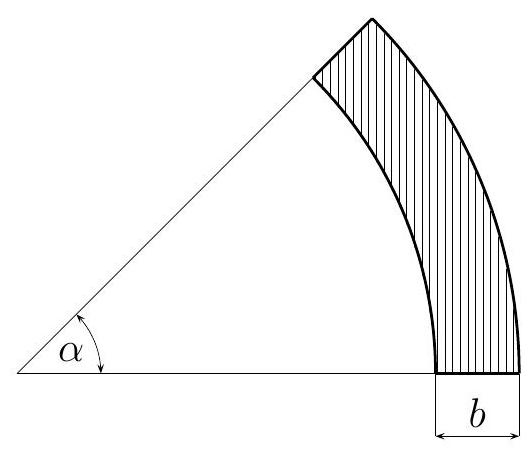
\includegraphics[max width=\textwidth, center]{2024_11_16_48a1022099522e94246ag-16}\\
stożka ściętego i promień kuli opisanej na nim. Podać wynik liczbowy dla $\alpha=\frac{\pi}{4}, b=4 \mathrm{~cm}$.
\end{enumerate}

\end{document}